% ---------
% --------
%!TEX TS-program = pdflatex
%!TEX encoding = UTF-8 Unicode
%!TEX spellcheck = English (Aspell)

\documentclass[11pt]{article}
\usepackage{lucy,handout,graphicx}
\usepackage{fourier-orns}
\usepackage{mathtools}
\usepackage[normalem]{ulem} % either use this (simple) or
\usepackage{tikz}

\def\Cdot{\mathbin{\text{\normalfont \textbullet}}}
\def\Sym#1{\texttt{\color{BrickRed}#1}}
\def\BlueSym#1{\textbf{\texttt{\color{RoyalBlue}#1}}}
\allowdisplaybreaks

\begin{document}

\begin{center}
\Large\textbf{CSCI 332, Fall 2026}%
\\
\LARGE\textbf{Homework 6}%
\\[0.5ex]
\large Due Monday, October 5 Anywhere on Earth (6am Tuesday)
\end{center}

\bigskip
\hrule
\bigskip

\subsection*{Submission Requirements}
\begin{itemize}
    \item Type or clearly hand-write your solutions into a PDF format so that they are legible and professional. Submit your PDF on Gradescope. 
    \item Do not submit your first draft. Type or clearly re-write your solutions for your final submission. If your submission is not legible, we will ask you to resubmit.
    \item Use Gradescope to assign problems to the correct page(s) in your solution. If you do not do this correctly, we will ask you to resubmit.
\end{itemize}

\subsection*{Academic Integrity}

Remember, you may access \EMPH{any} resource in preparing your solution to the homework. However, you \EMPH{must}
\begin{itemize}
    \item write your solutions in your own words, and
    \item credit every resource you use (for example: ``Bob Smith helped me on
    this problem. He took this course at UM in Fall 2020''; ``I found a solution
    to a problem similar to this one in the lecture notes for a different
    course, found at this link: www.profzeno.com/agreatclass/lecture10''; ``Here is a link to the full transcript of my chat with ChatGPT about the problems on this HW''.)
    Ask if you need any clarifications about how to properly cite your sources!
\end{itemize}




\newpage
%----------------------------------------------------------------------
    
\headers{CSCI 332}{Homework 6 (due October 5)}{Fall 2026}


\begin{enumerate}
%\parindent 1.5em \itemsep 4ex plus 0.5fil

%----------------------------------------------------------------------

\item (0 points) List the resources you used for each problem in this homework. If you used no resources except
lecture notes and videos and the linked textbook, you can say ``none''. If you used
an AI tool, you should put a link to your full conversation here, and you must
use the
\href{https://umaal.org/files/teaching/csci332_fall2026/agents.md}{provided
prompt}
 to guide the AI to act
as a tutor, not an answer-provider.

You will be asked to resubmit your homework if this section is blank.

Remember that no matter what resources you consulted, you must write your solutions
\emph{in your own words}.

\item (3 points) 
\begin{enumerate}
    \item
Recall the algorithm for binary search of sorted array $A[1..n]$
to find the index of a target element $t$, or $-1$ if it does not occur:

\begin{algo}
    \underline{BinarySearch(sorted $A[1..n]$, $t$):}\+ \\
    $\ell = 1, r = n$\\
    while $\ell \leq r$: \+ \\
    $m = \floor{\frac{\ell + r}{2}}$\\
    if $A[m] > t$: \Comment{go left}\+ \\
    $r = m - 1$ \- \\
    else if $A[m] < t$: \Comment{go right} \+ \\
    $\ell = m + 1$ \-\\
    else: \Comment{equal}\+ \\
    return $m$\- \- \- \\
    return $-1$
\end{algo}

In the worst case, how many times does the while loop execute? Give a $\Theta$ bound.

\item

    Now consider another problem regarding arrays: suppose you are given an array
    $A[1..n]$. It is not (necessarily) sorted, but it has another property: it alternates
    even and odd integers, except at one spot, where two even integers are adjacent.
    For example, in the array below, $88$ and $62$ are the adjacent even integers;
    notice that every other adjacent pair contains one even and one odd.

    \begin{center}
        
    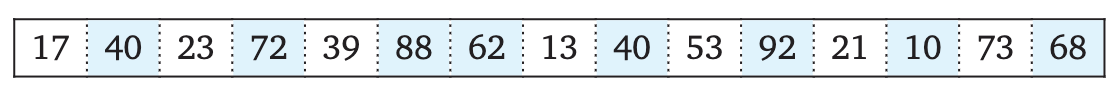
\includegraphics[width=.8\textwidth]{alternating_array.png}
    \end{center}

    Give an $O(\log n)$ time algorithm to find the index $i$ that starts the even pair;
    that is, the index $i$ so that $A[i] + A[i+1]$ is even. (Recall that that the sum of integers that are both even are even, whereas the sum of
    integers where one is even and one is odd is odd.) In the example above, $i=6$.

    The array may start either with an even or odd integer, but it satisfies the properties listed
    above.
\end{enumerate}

\item (7 points) Describe recursive algorithms for the following variants of the text
segmentation problem. Assume that you have a subroutine $\textsc{IsWord}$
that takes an array of characters as input and returns $\textsc{True}$
if and only if that string is a word.
\begin{enumerate}
    \item Given an array $A[1..n]$ of characters, compute the
    number of unique partitions of $A$ into words. For example,
    given the string \Sym{ARTISTOIL}, your algorithm should
    return 2, for the partitions \Sym{ARTIST OIL} and \Sym{ART IS TOIL}.
    \item Given two arrays $A[1..n]$ and $B[1..n]$ of characters,
    decide whether $A$ and $B$ can be partitioned into words at
    the same indices. For example, the strings \Sym{BOTHEARTHANDSATURNSPIN}
    and \Sym{PINSTARTRAPSANDRAGSLAP} can be paritioned into words
    at the same indices as follows:
    \begin{center}
        \Sym{BOT HEART HAND SAT URNS PIN}\\
        \Sym{PIN START RAPS AND RAGS LAP}
    \end{center}
    \item Given two arrays $A[1..n]$ and $B[1..n]$ of characters,
    compute the number of different ways that $A$ and $B$ can be
    partitioned into words at the same indices.

\end{enumerate}

\end{enumerate}
%%%%%%%%%%%%%%%%%%%%
\end{document}
